%%%%%%%%%%%%%%%%%%%%%%%%%%%%%%%%%%%%%%%%%%%%%%%%%%%%%%%
% A template for Wiley article submissions.
% Developed by Overleaf. 
%
% Please note that whilst this template provides a 
% preview of the typeset manuscript for submission, it 
% will not necessarily be the final publication layout.
%
% Usage notes:
% The "blind" option will make anonymous all author, affiliation, correspondence and funding information.
% Use "num-refs" option for numerical citation and references style.
% Use "alpha-refs" option for author-year citation and references style.

\documentclass[alpha-refs]{wiley-article-04t}
% \documentclass[blind,num-refs]{wiley-article}

% Add additional packages here if required
\usepackage{siunitx}

% For figures
\usepackage{graphics}

%For captions - even though template has complex caption commands
\usepackage[labelfont=bf,justification=centering]{caption}
\usepackage[font=small,labelfont=bf]{subcaption}
\captionsetup[sub]{font=tiny,labelfont={bf,sf}}

%% For figures numbered by section
\usepackage{chngcntr}
\counterwithin{figure}{section}
\counterwithin{table}{section}

%% Additional links for hyperref
\usepackage[unicode=true,pdfusetitle,
 bookmarks=false,bookmarksnumbered=false,bookmarksopen=true,bookmarksopenlevel=2,
 breaklinks=false,pdfborder={0 0 1},backref=false,colorlinks=false]
 {hyperref}
\hypersetup{pdfstartview={XYZ null null 1}}

\usepackage[backend=bibtex,
			natbib=true, 
			style=chicago-authordate]{biblatex}
\addbibresource{wp4.bib}

\usepackage{array}
\usepackage{longtable}
%\usepackage{fullpage}

\usepackage{lmodern}
\newcommand{\graph}[3]{
\raisebox{-#1mm}{\includegraphics[height=#2em,width=3cm]{#3}}
}

\usepackage{booktabs} % for vertically partitioned table

\usepackage{lipsum}  % for fillers

% Additional
\usepackage{amsmath}
\usepackage{tabularx}
\usepackage{tabulary}
\usepackage{float}
\usepackage[flushleft]{threeparttable}
%%%%%%%%#################################################################################%%%%%%%%%%%%%%%%%%%%%%%%%%%%%

% Update article type if known
\papertype{WORLD BANK EDUCATION GLOBAL PRACTICE}
% Include section in journal if known, otherwise delete
\paperfield{Russian Federation: Analytical Services and Advisory Activity: 
P170978}

\title{Returns to Education in the Russian Federation: Application of a machine learning instrumental variable technique for policy development in priority regions}

% List acknowledgements here.
\fundinginfo{Thanks are due to the Higher School of Economics, Moscow for making the Russian Longitudinal Monitoring Study (RLMS) Household data readily available for reseachers around the world. The code used for this paper is made freely available for all researchers at \url{https://bitbucket.org/zagamog/edreru/src/master/}}

% Include full author names and degrees, when required by the journal.
% Use the \authfn to add symbols for additional footnotes and present addresses, if any. Usually start with 1 for notes about author contributions; then continuing with 2 etc if any author has a different present address.

\author[*]{Ekaterina Melianova}
\author[*]{\hspace{-1em}Suhas Parandekar}
\author[*]{\hspace{-1em}Harry Patrinos}
\author[*]{\hspace{-1em}Art\"{e}m Volgin}

% List abbreviations here, if any. Please note that it is preferred that abbreviations be defined at the first instance they appear in the text, rather than creating an abbreviations list.
\acks{\begin{normalsize}
\emph{Country Director:} Renaud Seligman; \emph{Regional Director:} Fadia Saadah; \emph{Practice Manager:} Harry Patrinos; \emph{Program Leader:} Dorota Nowak; \emph{Peer Reviewers}: Cristian Aedo; Ruslan Yemtsov; Husein Abdul-Hamid; \emph{Team members:} Polina Zavalina; Zhanna Terlyga. Thanks to seminar participants at the World Bank Moscow office on Jan. 29, 2020 for useful feedback. Any errors are a responsibility of the authors.
\end{normalsize}
\vspace{-0.2in}}

%\contrib[\authfn{1}]{Equally contributing authors.}

% Include full affiliation details for all authors
\affil[*]{Education Global Practice, Europe and Central Asia}

%\corraddress{Author One PhD, Department, Institution, City, State or Province, Postal Code, Country}
\corremail{sparandekar@worldbank.org}

%\presentadd[\authfn{2}]{Department, Institution, City, State or Province, Postal Code, Country}

% Include the name of the author that should appear in the running header
\runningauthor{P170978: WP04 - Machine Learning Post Lasso IV Priority Regions}

\begin{document}

\maketitle

\begin{abstract}
This is a generic template designed for use by multiple journals, which includes several options for customization. Please consult the author guidelines for the journal to which you are submitting in order to confirm that your manuscript will comply with the journal's requirements. Please replace this text with your abstract.

% Please include a maximum of seven keywords
\keywords{keyword 1, \emph{keyword 2}, keyword 3, keyword 4, keyword 5, keyword 6, keyword 7}
\end{abstract}


\section{Motivation for this paper}

\subsection{Stylized fact 1: Returns trend and looking at cohorts}

\subsection{Stylized fact 2: Priority regions and policy options for education}

\lipsum[1]

\section{Literature Review: Use of Instrumental Variables in Returns to Education Studies}

General Literature


Russia Specific


The usage of instrumental variables as a way of correcting for the endogeneity of educational attainments in the estimation of returns to schooling in Russia is relatively rare. Nevertheless, there are several papers that leveraged IV technique and made a number of important conclusions.

One research ascertained that during the transition returns to education in Russia were not improving and remained among the most deficient in the world \citep{cheidvasser_educated_2007}. The researchers instrumented years of schooling, employing a policy experiment in Russia from the 1950s to 1960s, and corrected for a selectivity bias by adding an equation for the labor market participation. It was highlighted that the excess of well-educated workers seemed to be the main underpinning factor of wage differentials in Russia after Soviet Union dissolution. Additionally, the study showed that heterogeneity in rates of returns to education in Russia also hails from gender differences similar to the global patterns: women receive greater returns to higher education than men.

Utilizing the same instruments as \citet{cheidvasser_educated_2007}, \citet{akhmedjonov_higher_2011} evaluated the magnitude of the education premiums in Russia between 2000 and 2002. Both OLS and 2SLS estimates (8\% and 19.1\% respectively) were indicative of significant returns and the formation of a more flexible wage structure in the Russian Federation.

\citet{arabsheibani_returns_2012} introduced the age of sexual intercourse as another instrumental variable to tackle endogeneity in schooling. In line with some past research, the scholars show that OLS undervalues returns to education compared to the IV estimates. The study adopts an instrumental variable quantile approach over the wage distribution in addition to the conditional mean estimation.

\citet{kyui_expansion_2016}, using the amount available slots as an instrument, showed that returns to schooling in Russia declined for those who took advantage of higher education expansion in a post-communist Russia (1990-2005) in comparison to youths who obtained university degree in preceding periods. In an earlier study, \citet{kyui_returns_2010} used the accessibility of tertiary education and the education levels of other household members as instruments in a wage equation (2010). The scholar demonstrated that a growth in returns to education in the Russian Federation does not indicate its closeness to the developed countries \citep{kyui_returns_2010}.

\citet{belskaya_college_2014} evaluated a large-scale college expansion in Russia after the breakdown of the Soviet Union (2014). Using the number of campuses in the municipality of residence at age 17 as an instrument, the research contended that as the number of university campuses grew, individuals with low returns to schooling grew as well. But for a marginal person, who switched into a treatment group as a result of new campuses opening, the total gains from attending a college are considerable and positive. Furthermore, the scholars found that students with higher returns are attracted more intensively by new campuses opened in constrained municipalities (small non-capital cities or those lacking higher education institutions before college expansion) in comparison to the unconstrained ones.


\section{Lasso and Post-Lasso Instrumental Variables: Overview of Estimation Method}

This study considers post-Lasso IV estimation procedure, which was elaborated by \citet{belloni_high_2011} and \citet{belloni_sparse_2012} a decade ago. The method performs an optimal IV selection, using the Lasso statistical learning algorithm.

The Lasso (Least Absolute Shrinkage and Selection Operator) is a regression analysis method, which was popularized by \citet{tibshirani_regression_1996}. As it stems from the name, the method does both variable selection and shrinkage (unlike Ridge, which only shrinks). The Lasso solves a regression problem with L1 penalization of finding \citep{diebold_econometric_2019}:

\begin{equation}\hat{\beta}_{L A S S O}=\operatorname{argmin}_{\beta}\left(\sum_{i=1}^{N}\left(y_{i}-\sum_{i} \beta_{i} x_{i t}\right)^{2}+\lambda \sum_{i=1}^{K}\left|\beta_{i}\right|\right)
\end{equation}

or equivalently:

\begin{equation}\hat{\beta}_{L A S S O}=\operatorname{argmin}_{\beta} \sum_{i=1}^{N}\left(y_{i}-\sum_{i} \beta_{i} x_{i t}\right)^{2}\end{equation}

s.t.

\begin{equation}\sum_{i=1}^{K}\left|\beta_{i}\right| \leq c\end{equation}

\noindent
where $y$ and $x$ are dependent and independent variables for $i = 1,2,...,N$, respectively; $\beta$ is a regression coefficient of interest; $\lambda$ is a tuning parameter, $K$ is the number of degrees of freedom (d.f.) in the model fitting, $t$ is the amount of independent variables.

The equations portray that the Lasso loss function is composed of the least squares estimator (or can be extended to many other estimators) and a penalty term in a form of the absolute coefficient value. The main distinctive property of this technique is the ability to conduct feature selection procedure by nullifying regression coefficients of low importance, which is of particular relevance in situations with large feature sets. In case of zero lambda, the method gets back to OLS, while huge lambdas reduce coefficients to zero and may lead to under-fitting.

The d.f. results of Lasso are convenient: the effective number of parameters equals exactly to the number of the picked up (non-zero) variables. The best-fitting lambda can be chosen by reliance on various information criteria (e.g., AIC and SIC) or cross-validation. The additional advantage of the Lasso algorithm is its relative computational tractability due to the convex minimization problem \citep{diebold_econometric_2019}.

The post-Lasso was devised for the instrument selection by excluding IVs with insignificant effects on the endogenous variable. Particularly, the post-Lasso algorithm consists of 2 steps: (1) IV selection in the first-stage regression using Lasso, (2) 2SLS estimation with the picked up instruments. The method allows to enhance the precision of inferences due to the advantage of implementing multiple instruments and avoiding the finite sample bias expansion. As long as the instruments of economic importance are filtered out, the erroneous exclusion of valid instrument with minor effects does not amend the 2SLS estimation \citep{belloni_high-dimensional_2014}. This is achieved due to the assumption that the conditional mean of a given endogenous attribute can be well approached by a small range of key instruments.

The Two-Stage Least Squares specification of interest in the present paper can be written by the following equations.

First stage:

\begin{equation}
x_{1i}=z_{i}^{\prime} \pi_{1}+x_{2i}^{\prime} \pi_{2}+v_{i}
\end{equation}

Second stage:

\begin{equation}
y_{i}=x_{1 i} \beta_{1}+x_{2i}^{\prime} \beta_{2}+\varepsilon_{i}
\end{equation}

\noindent
where $y$ is a logarithm of wages for $i = 1,2,...,N$; $x_{1i}$ reflects years of education (an endogenous regressor); $x_{2i}$ is a vector of exogenous variables: labor market experience and its squared term; $z_{i}$ is a vector of instrumental variables, aggregated at a regional level in the Russian Federation: the number of higher education institutions, high school graduate students per school, standard deviation from the national average EGE scores (Russian school-leaving examination), net migration rate, women to men ratio, marriage rate, employment in female-dominated industries, and literacy level in 1897 in the Russian empire; $\beta_{1}$ is the causal effect of $x_{1}$ an $y$; $\varepsilon_{i}$ and $v_{i}$ are normally distributed error terms.

When a specified 2SLS model contains exogenous regressors, the Lasso selection technique is applied over the transformed first-stage equation where each side is multiplied by a projection matrix of control variables (i.e., they are partialed out). Then the Lasso estimator is given by: 

\begin{equation}\hat{\pi}_{1}^{\text {Lasso}}=\arg \min_{\pi_{1}}\left\{\frac{1}{N} \sum_{i=1}^{N}\left(x_{1 i}^{*} -z_{i}^{*} \pi_{1}\right)^{2} +\frac{\lambda}{N}\left\|\pi_{1}\right\|_{1}\right\}\end{equation}

\noindent
where $x_{1}^{*}$ and $z^{*}$ are the projected endogenous regressor (education years) and IVs, respectively; $\pi_{1}$ is a regression coefficient of interest; $\lambda$ stands for the regularization parameter.


\section{Empirical Studies using Post-Lasso IV methodology}

\lipsum[5]

\section{Findings 1: Traditional Instrumental Variable Technique}

Figure \ref{fig:5.1} displays correlations between the instrumental variables and years of education by cohorts and figure \ref{fig:5.2} is a correlation matrix between all the region-level instruments of focus: the number of higher education institutions \textit{(HSGPER)}, high school graduate students per school \textit{(high\_n)}, standard deviation from the national average EGE scores \textit{(s1z)}, net migration rate \textit{(migrationrate)}, women to men ratio \textit{(women2menratio)}, marriage rate \textit{(marriagerate)}, employment in female-dominated industries \textit{(migrationrate)}, and literacy level in 1897 in the Russian empire \textit{(Literacy\_97)}.


\begin{figure}[h]
	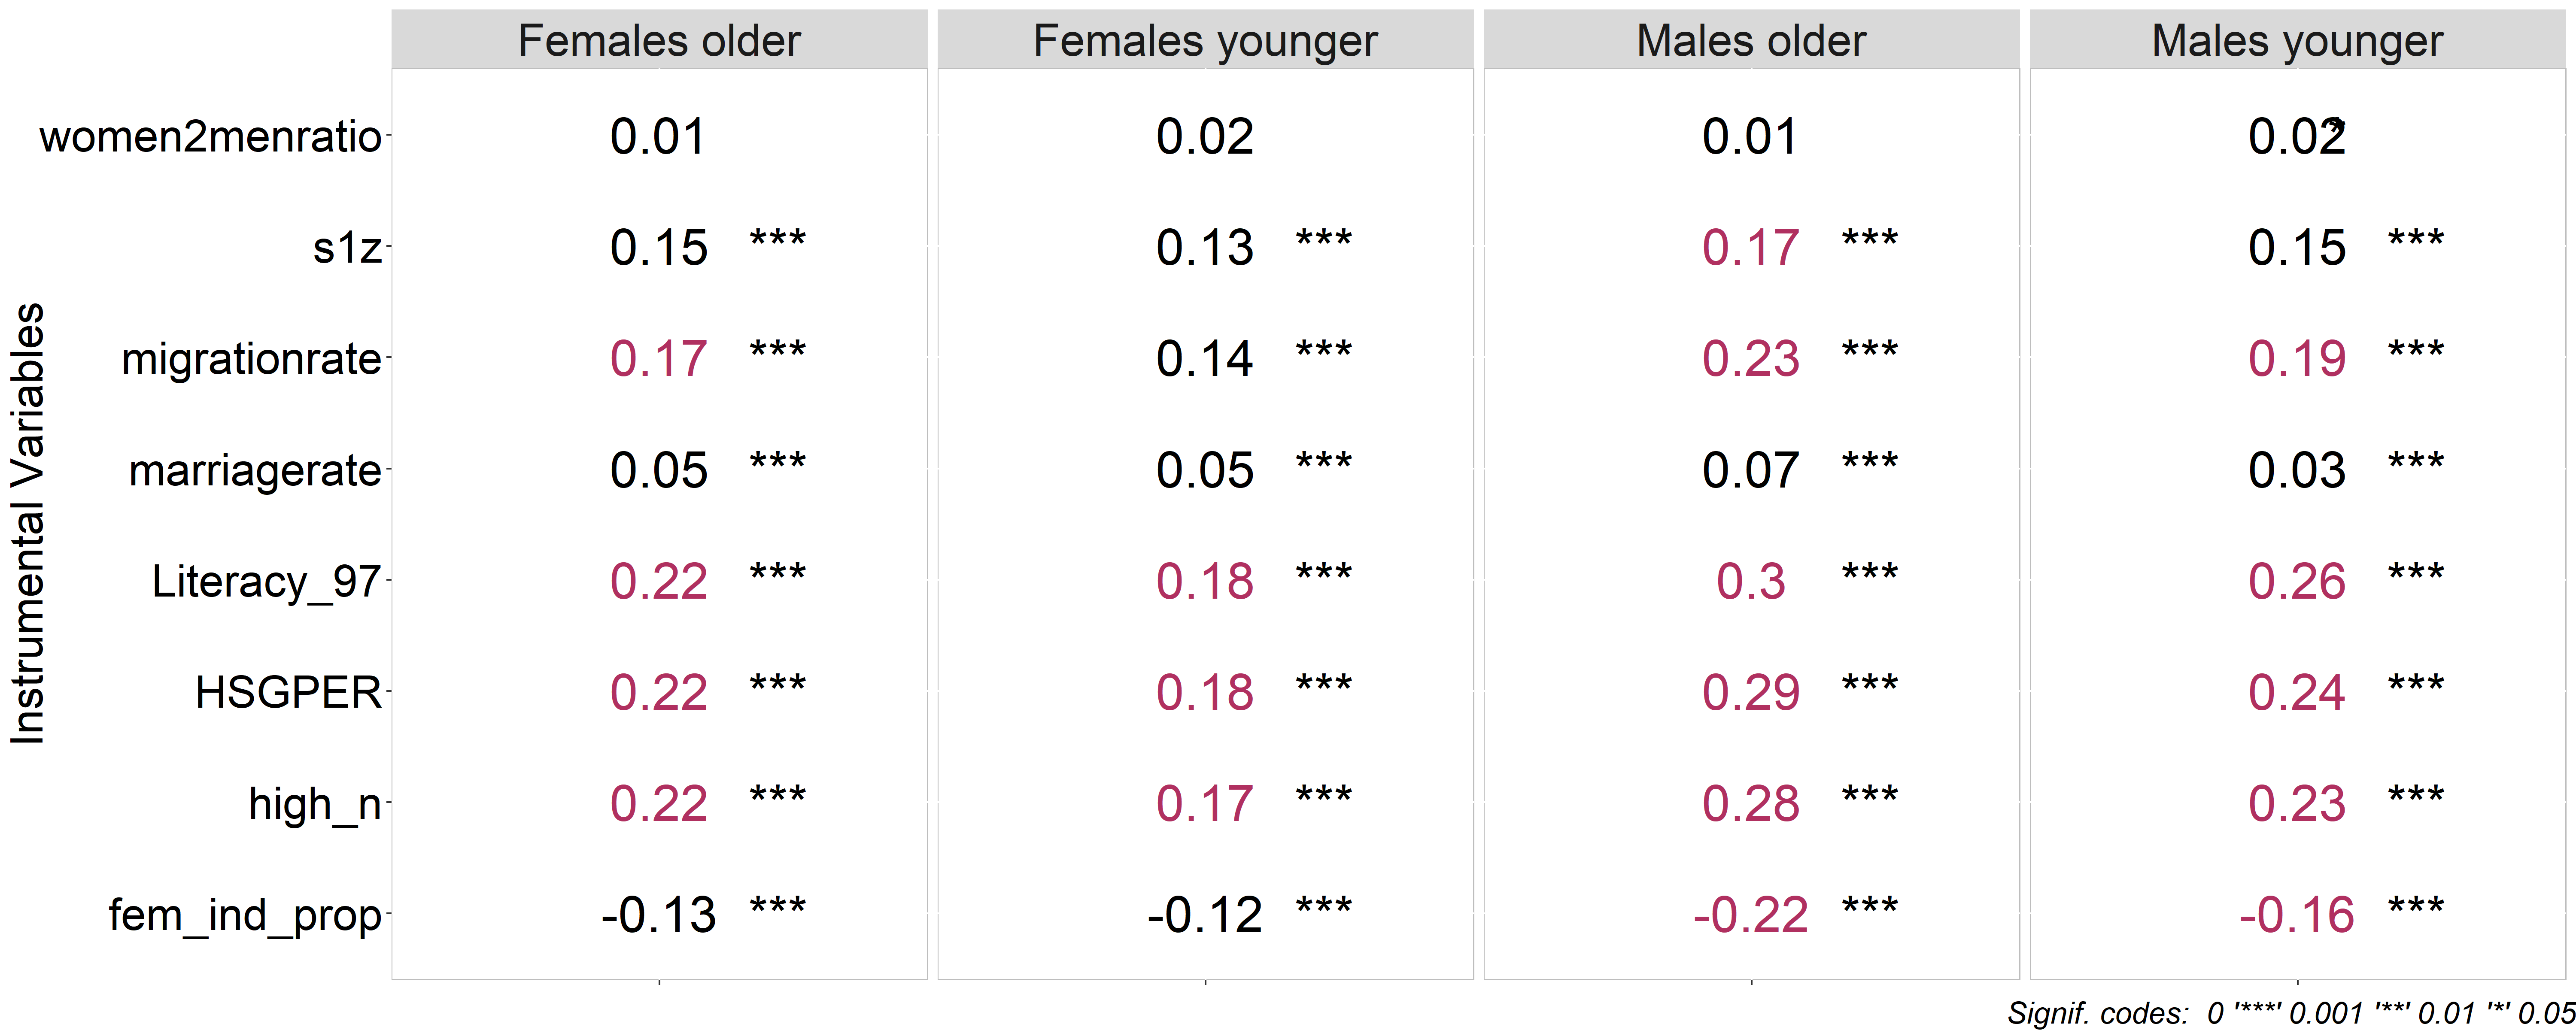
\includegraphics[width=\textwidth]{cor_by_cohorts.png}
	\caption{Pearson correlation between Instrumental Variables and Years of Education by Cohorts, 2018} \label{fig:5.1}
\end{figure}

\begin{figure}[h]
	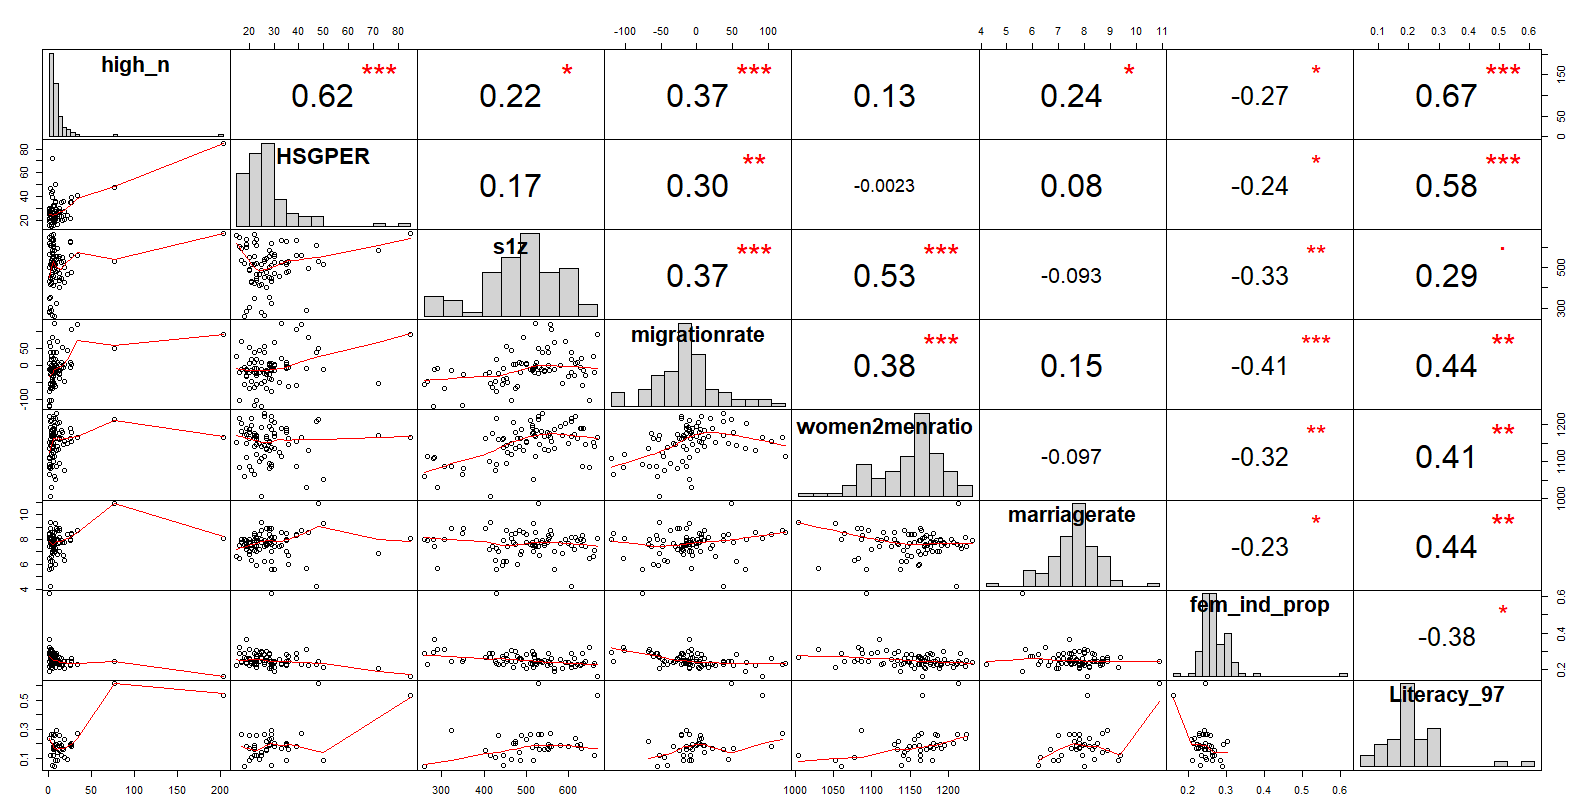
\includegraphics[width=\textwidth]{cor_matrix.png}
	\caption{Pearson correlation Matrix and Distributions for Instrumental Variables, 2018} \label{fig:5.2}
\end{figure}


\begin{table}[ht]
	\centering
	\caption{Individual 2SLS Estimates (Standard Errors) for each IV by Cohorts and OLS Results, 2018}
	\label{tab:5.1}	
	\resizebox{\textwidth}{!}{
\begin{tabular}{lcccccccc}
		\hline
		IVs & Female\_young & N1 & Female\_old & N2 & Male\_young & N3 & Male\_old & N4 \\ 
		\hline
		high\_n & 1.959 (0.229) & 9779 & 0.857 (0.042) & 11564 & 0.787 (0.047) & 10636 & 0.64 (0.026) & 9826 \\ 
		HSGPER & 1.717 (0.174) & 9779 & 0.887 (0.044) & 11564 & 0.754 (0.043) & 10636 & 0.636 (0.026) & 9826 \\ 
		s1z & 1.34 (0.195) & 9779 & 0.602 (0.041) & 11564 & 0.648 (0.06) & 10636 & 0.501 (0.034) & 9826 \\ 
		migrationrate & 1.429 (0.163) & 9779 & 0.796 (0.05) & 11564 & 0.625 (0.045) & 10636 & 0.534 (0.028) & 9826 \\ 
		women2menratio & -0.439 (0.609) & 9779 & -0.99 (0.731) & 11564 & -0.105 (0.154) & 10636 & -2.998 (5.602) & 9826 \\ 
		marriagerate & 2.312 (0.536) & 9779 & 2.18 (0.477) & 11564 & 2.638 (0.705) & 10636 & 1.988 (0.378) & 9826 \\ 
		fem\_ind\_prop & 1.677 (0.218) & 9779 & 0.985 (0.079) & 11564 & 0.829 (0.066) & 10636 & 0.663 (0.034) & 9826 \\ 
		Literacy\_97 & 1.868 (0.232) & 6834 & 0.912 (0.053) & 7860 & 0.726 (0.044) & 7247 & 0.641 (0.03) & 6701 \\ 
		\hline
		OLS & 0.092 (0.003) & 9775 & 0.107 (0.003) & 11560 & 0.103 (0.003) & 10632 & 0.114 (0.003) & 9822 \\ 
		\hline
\end{tabular}
}
\end{table}


\section{Findings 2: Post Lasso IV Results}

\begin{figure}[h]
	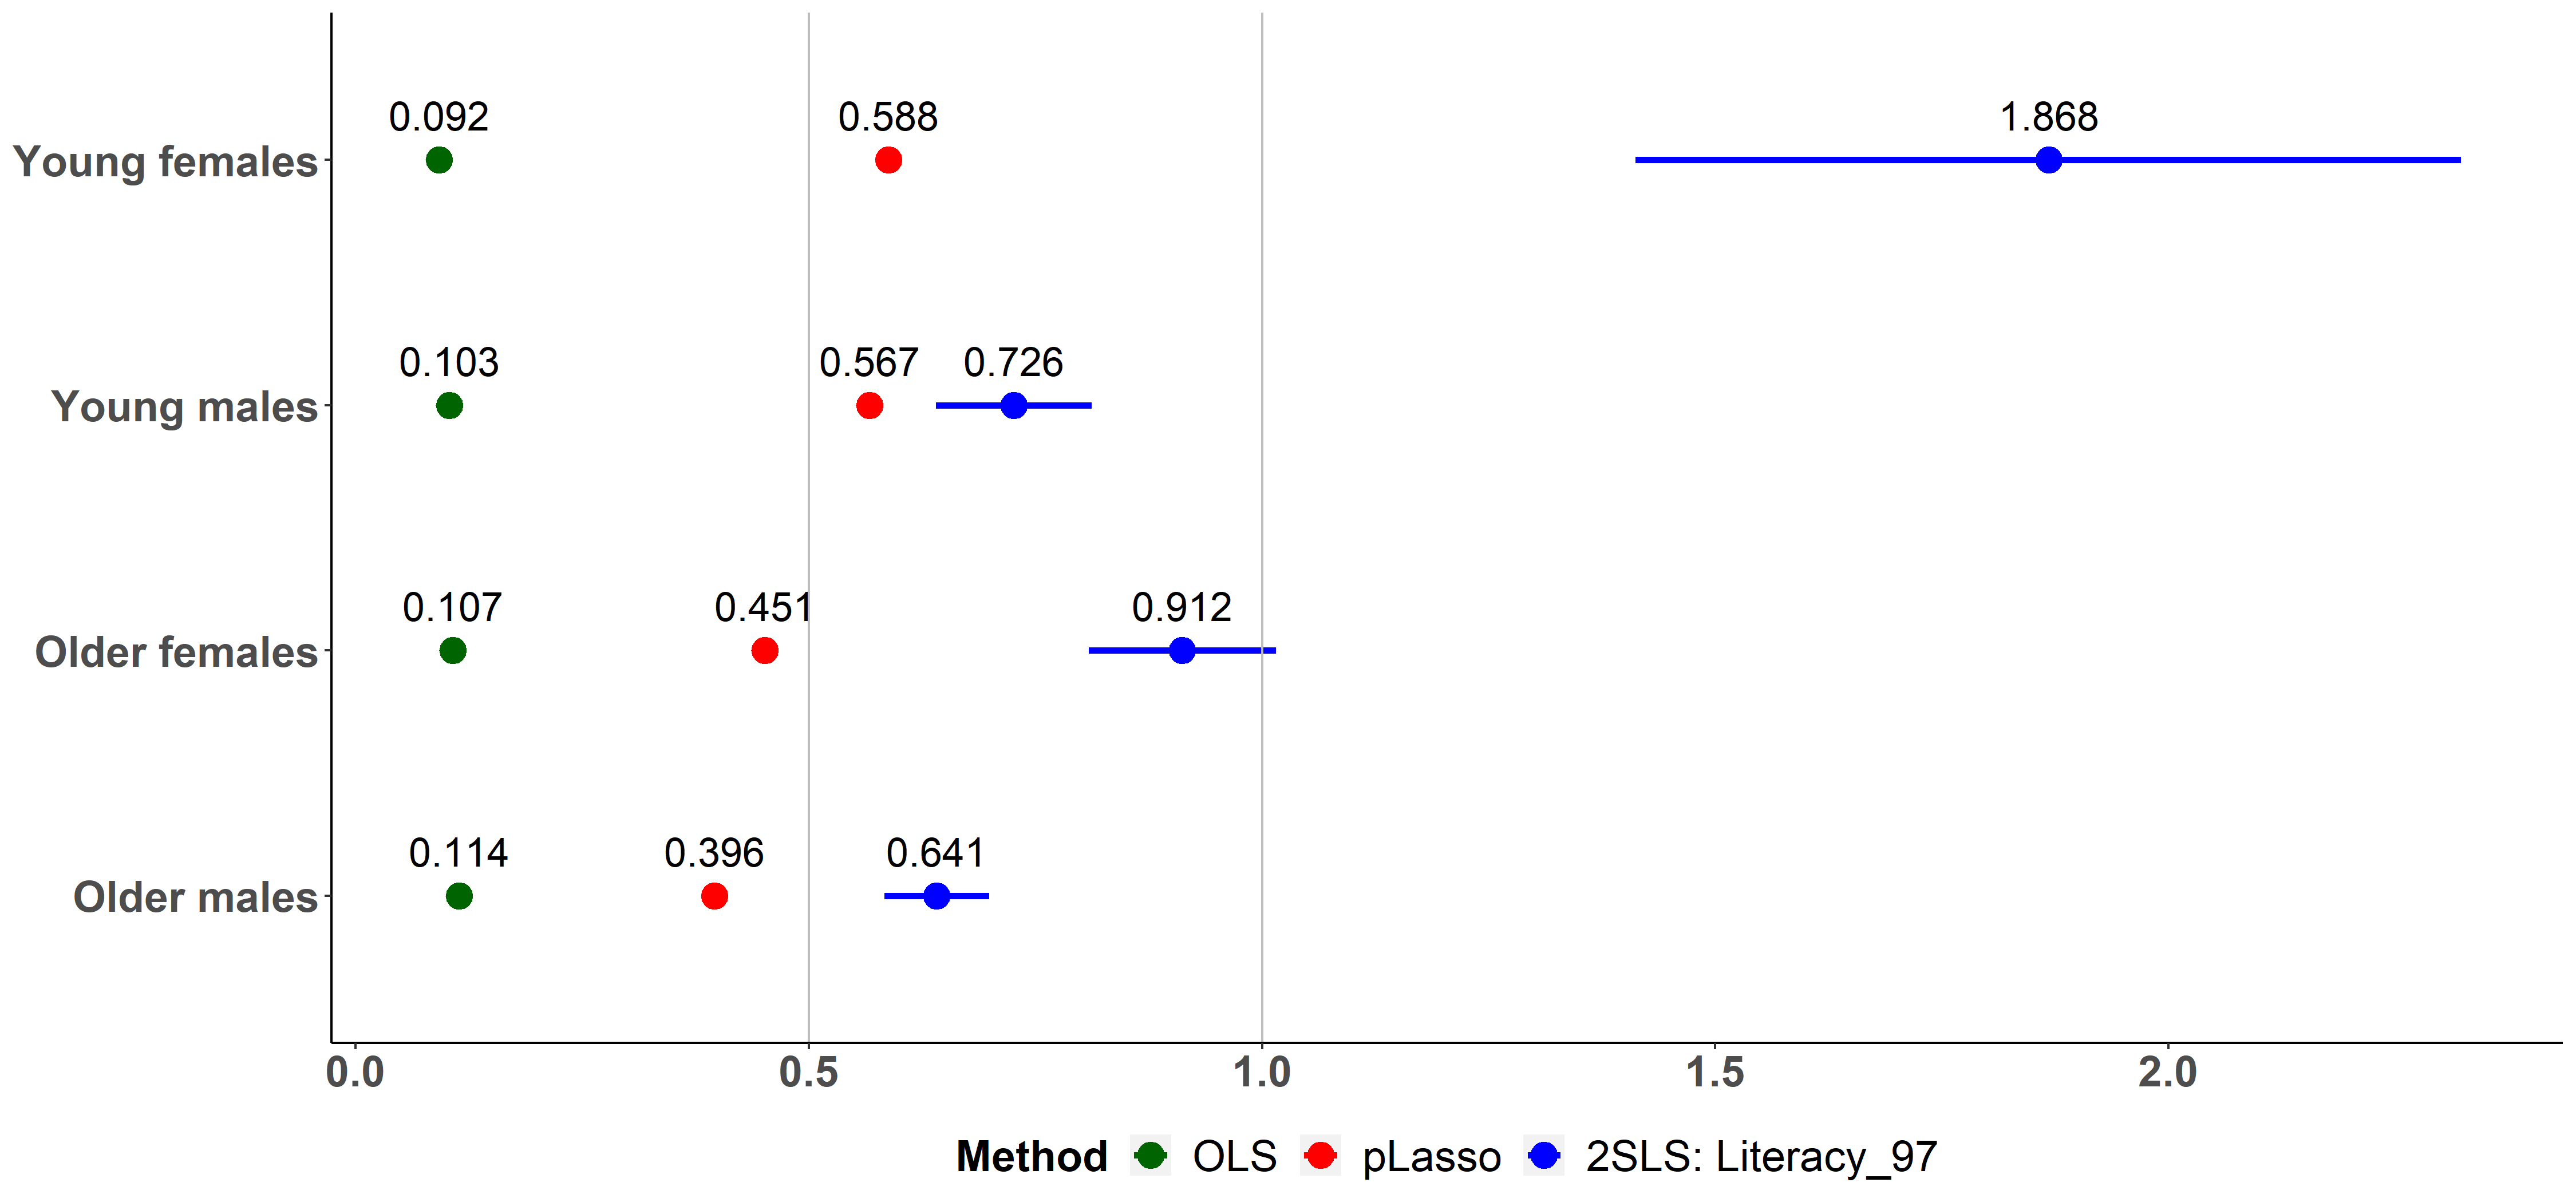
\includegraphics[width=\textwidth]{iv_3_methods.png}
	\caption{Returns to Education Estimates and 95\% CIs for Post-Lasso, 2SLS, and OLS by Cohorts, 2018} \label{fig:5.3}
\end{figure}

\begin{table}[H]
	\centering	
	\caption{Means and Standard Deviations for Education Years and Wages by Ranked Groups of Regions, 2018}
	\label{tab:5.2}	
	\resizebox{\textwidth}{!}{
		\begin{tabular}{llllll}
			\hline		Variable & Group & Top 20 & Middle 40 & Bottom 20 & Whole Sample \\ 
			\hline
			edu\_yrs & Female older & 13.38 (2.62) & 13.91 (2.73) & 13.91 (2.7) & 13.76 (2.71) \\ 
			&Female young & 14.09 (2.75) & 14.55 (2.66) & 14.8 (2.61) & 14.49 (2.68) \\ 
			&Male older & 12.51 (2.34) & 13.21 (2.66) & 13.26 (2.68) & 13.03 (2.6) \\ 
			&Male young & 13.04 (2.58) & 13.83 (2.74) & 14.02 (2.75) & 13.67 (2.73) \\ 
			wage & Female older & 19379.02 (11665.53) & 27784.51 (18811.94) & 26329.79 (16935.15) & 25132.36 (17104.73) \\ 
			&Female young & 19731.68 (10639.46) & 30433.91 (20443.96) & 27890.92 (16672.82) & 27170.08 (18149.23) \\ 
			&Male older & 26392.05 (18023.65) & 36872.17 (26937.81) & 35302.24 (24426.05) & 33650.33 (24684.13) \\ 
			&Male young & 31539.2 (18744.09) & 40202.54 (24260.45) & 37103.45 (24277.62) & 37266.07 (23242.51) \\
			\midrule
			Priority regions &  & \begin{tabular}[l]{@{}l@{}}Pskovskaya Obl.,\\ Resp. Karelia, \\Resp. Mariy El\end{tabular} & \begin{tabular}[l]{@{}l@{}}Altayskiy Kray, \\Kurganskaya Obl.,\\ Chuvashskaya Resp.,\\ Resp.a Altay \end{tabular}& \begin{tabular}[l]{@{}l@{}}Resp. Adygeya,\\ Resp. Kalmykiya,\\ Resp. Tyva \end{tabular}& \begin{tabular}[l]{@{}l@{}} Resp. Adygeya,\\ Pskovskaya Obl.,\\ Altayskiy Kray,\\ Kurganskaya Obl.,\\ Resp. Kalmykiya, \\ Chuvashskaya Resp.,\\ Res. Altay,\\ Resp. Karelia,\\ Resp. Tyva,\\ Resp. Mariy El \end{tabular}\\ 
			\hline
		\end{tabular}
}
\begin{tablenotes}
	\small
	\item \textit{Note: the ranking was based on the regional level of employment among vocational level holders.}
\end{tablenotes}
\end{table}


\begin{figure}[H]
	\begin{minipage}[b]{\linewidth}
		\centering
		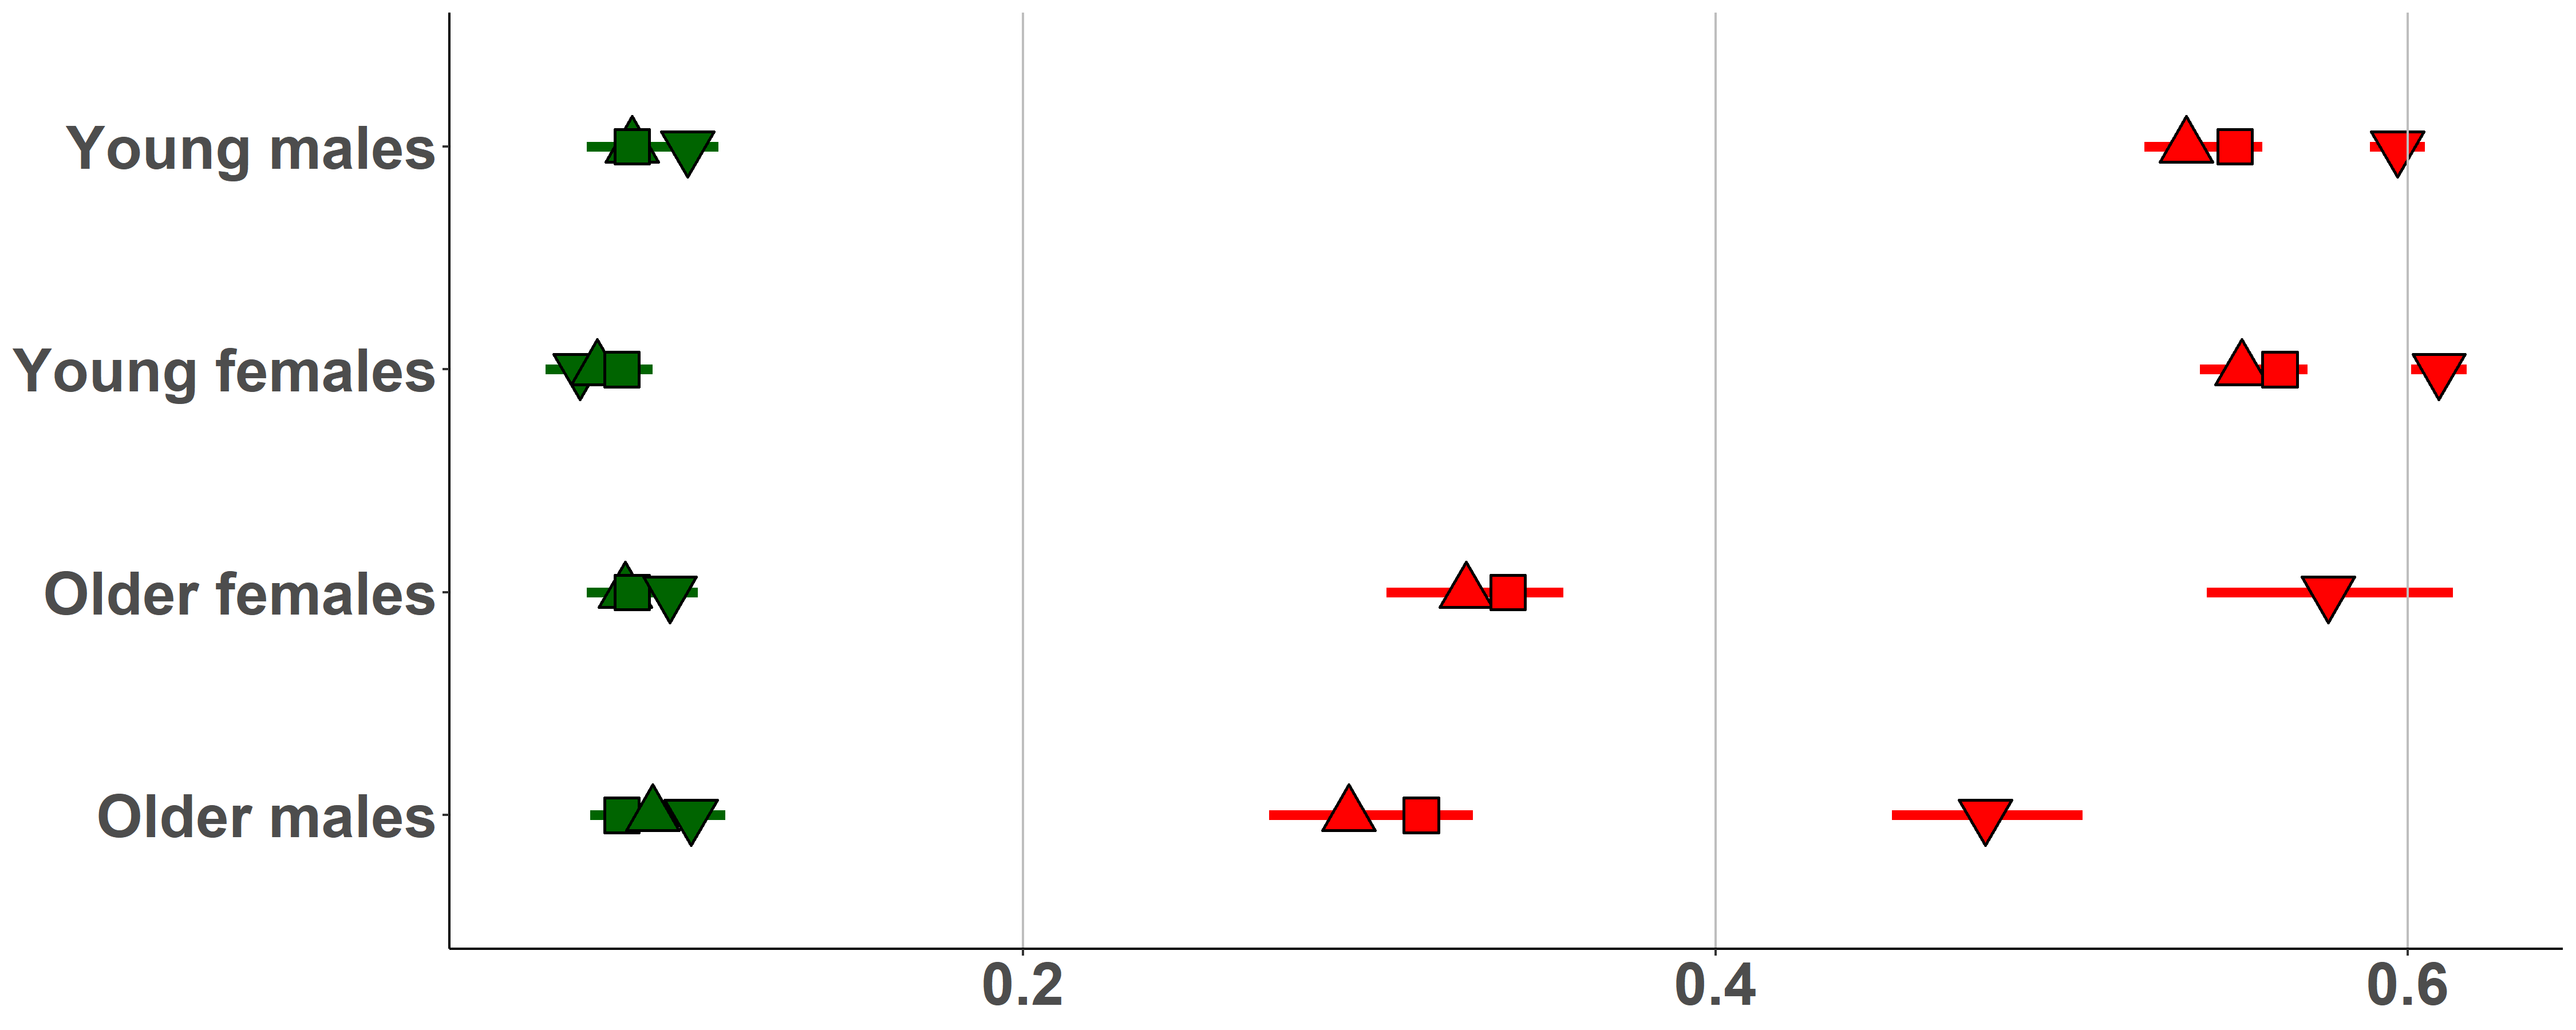
\includegraphics[width=350pt]{iv_2_methods_1.png}
		\subcaption{Ranking variable: regional percentage of vocational education as final level amongst women 25-64}\label{fig:5.4a}
	\end{minipage}
	\hfill
	\begin{minipage}[b]{\linewidth}
		\centering
		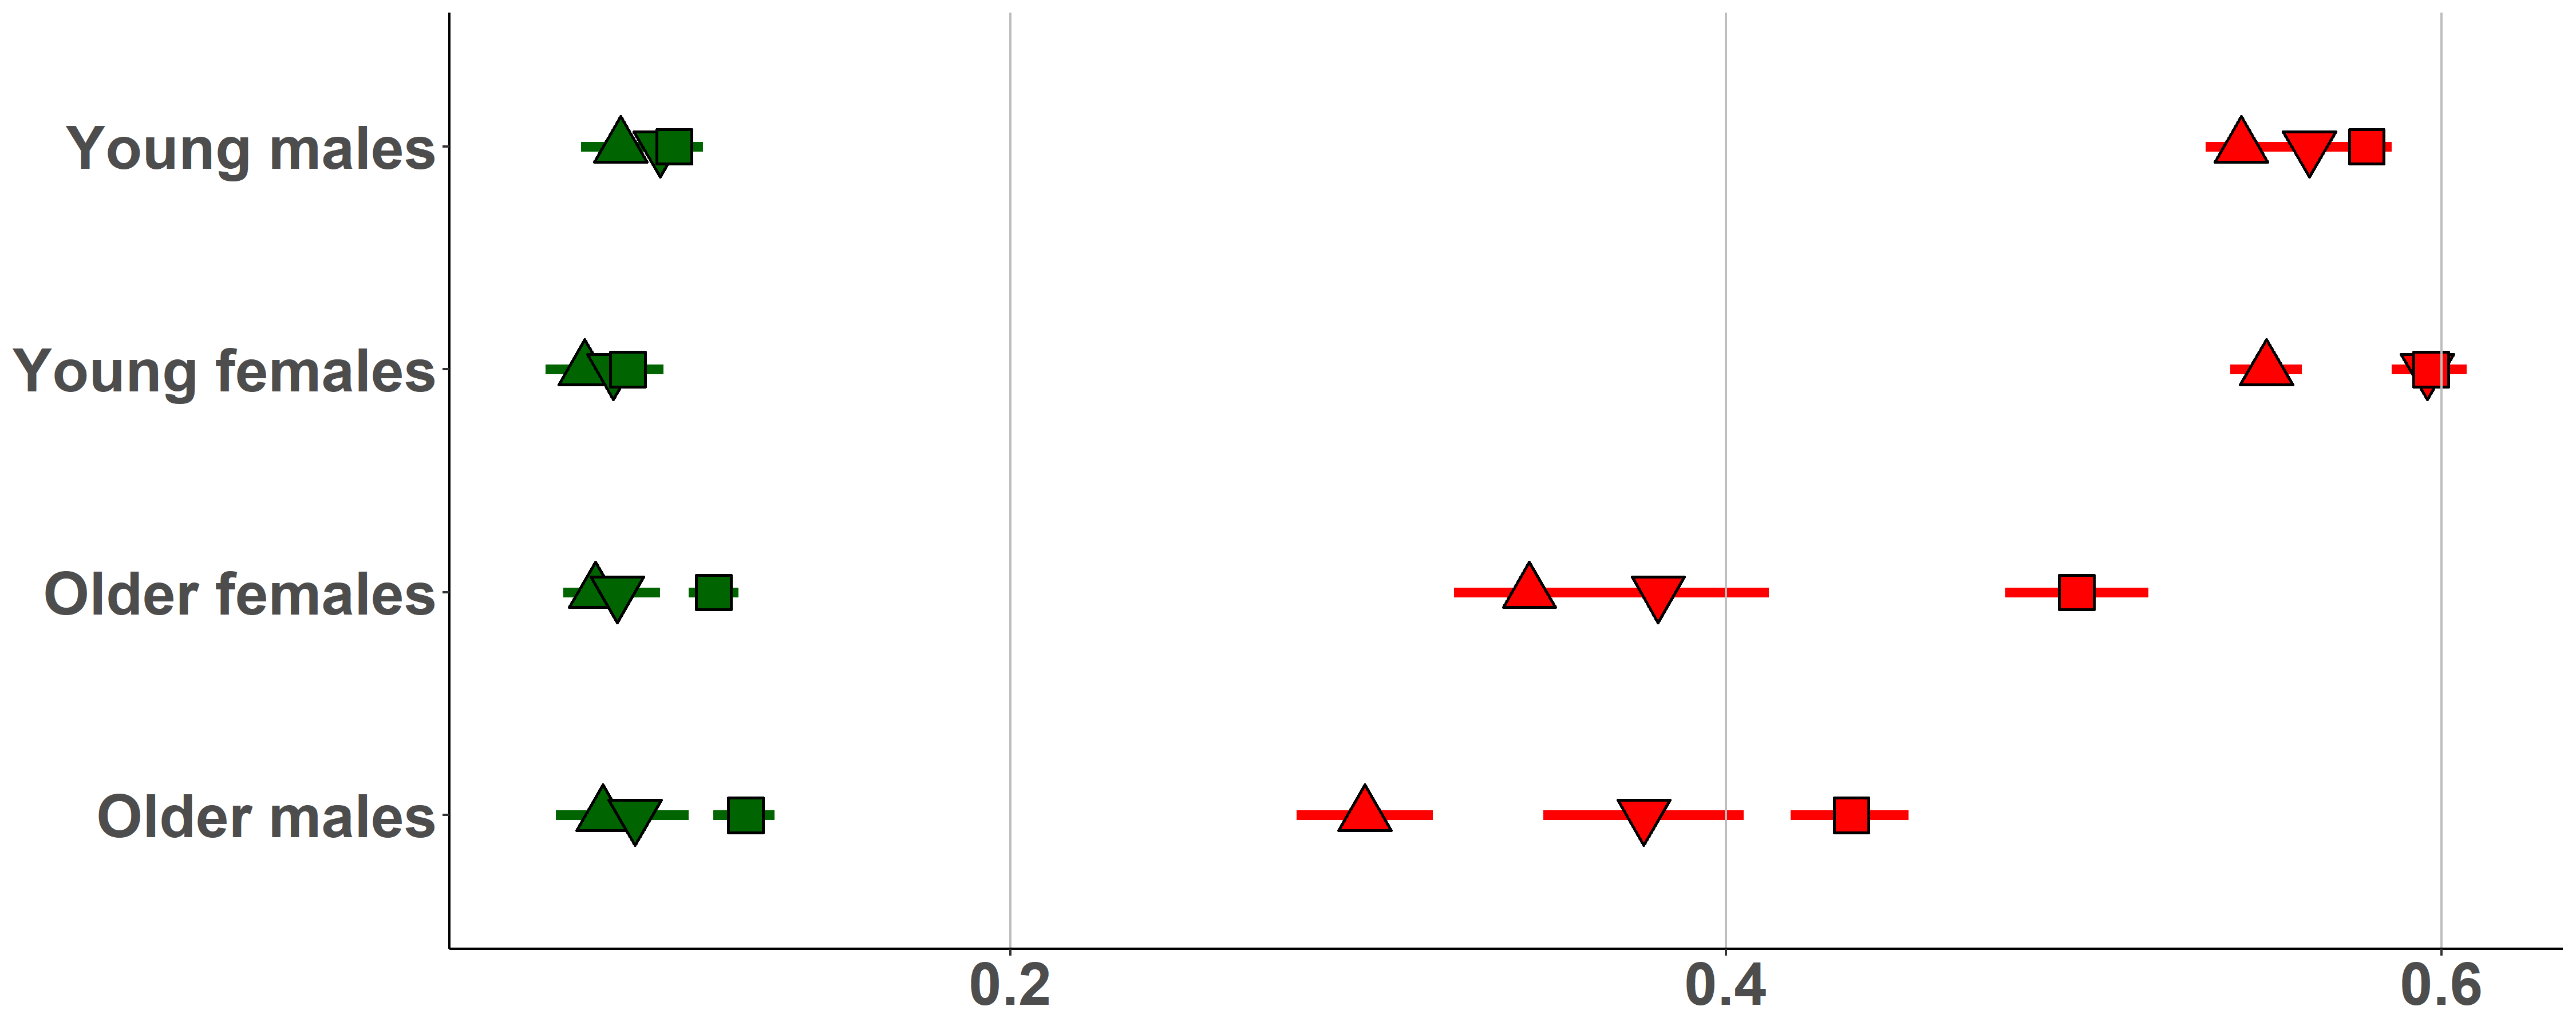
\includegraphics[width=350pt]{iv_2_methods_2.png}
		\subcaption{Ranking variable: regional level of employment among vocational level holders}\label{fig:5.4b}
	\end{minipage}
	\hfill
	\begin{minipage}[b]{\linewidth}
		\centering
		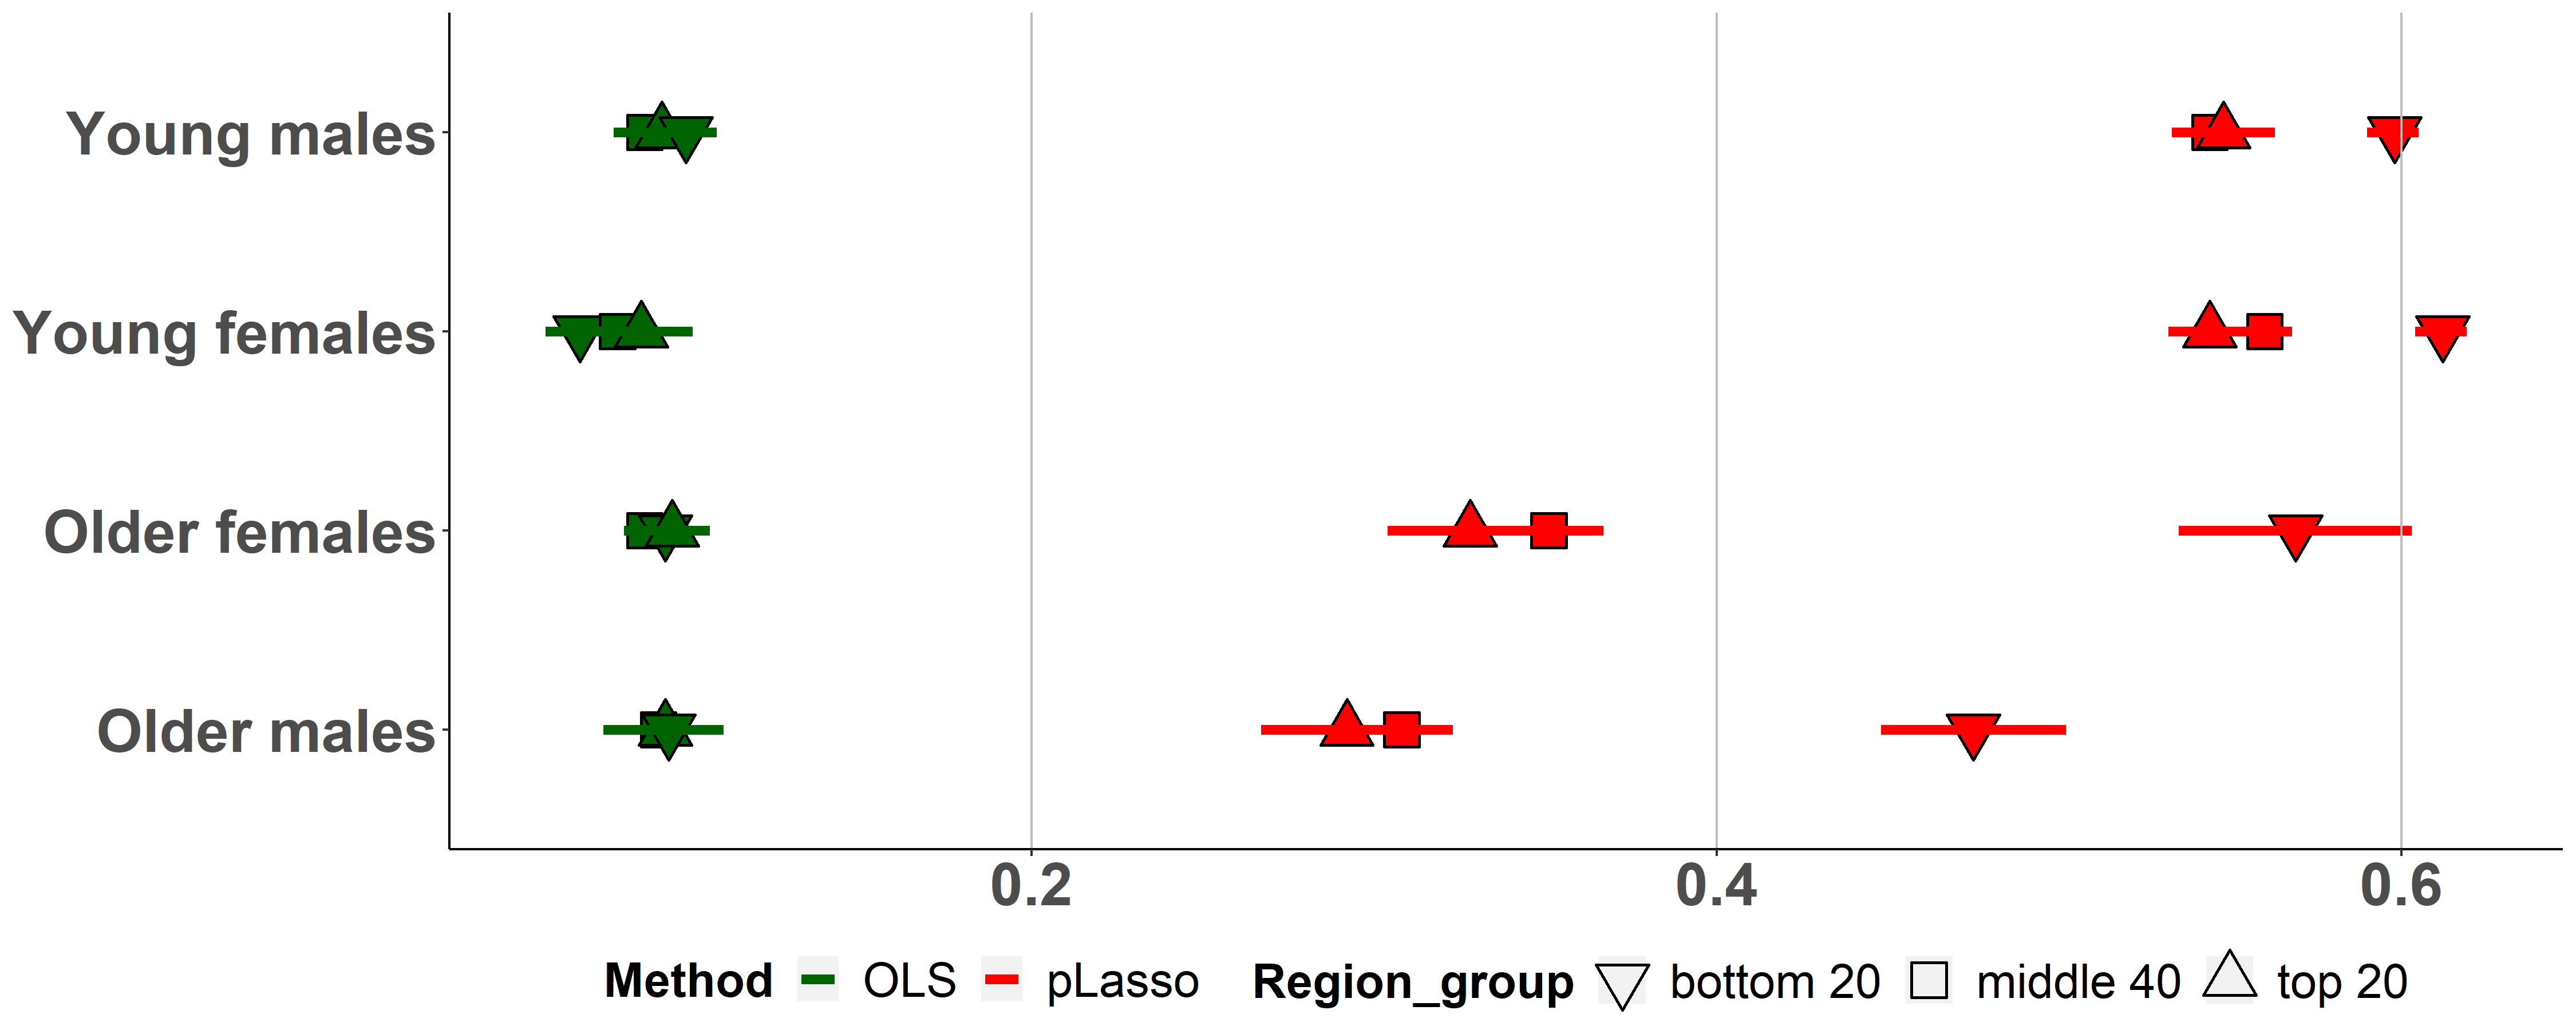
\includegraphics[width=350pt]{iv_2_methods_3.png}
		\subcaption{Ranking variable: regional employment level of vocational education holders \\
	    multiplied with reciprocal of employment level of higher education holders}\label{fig:5.4c}
	\end{minipage}
	\caption{Returns to Education Estimates and 95\% CIs for Post-Lasso and OLS by Cohorts and Ranked Groups of Regions, 2018}
	\label{fig:5.4}
\end{figure}


\begin{figure}[H]
	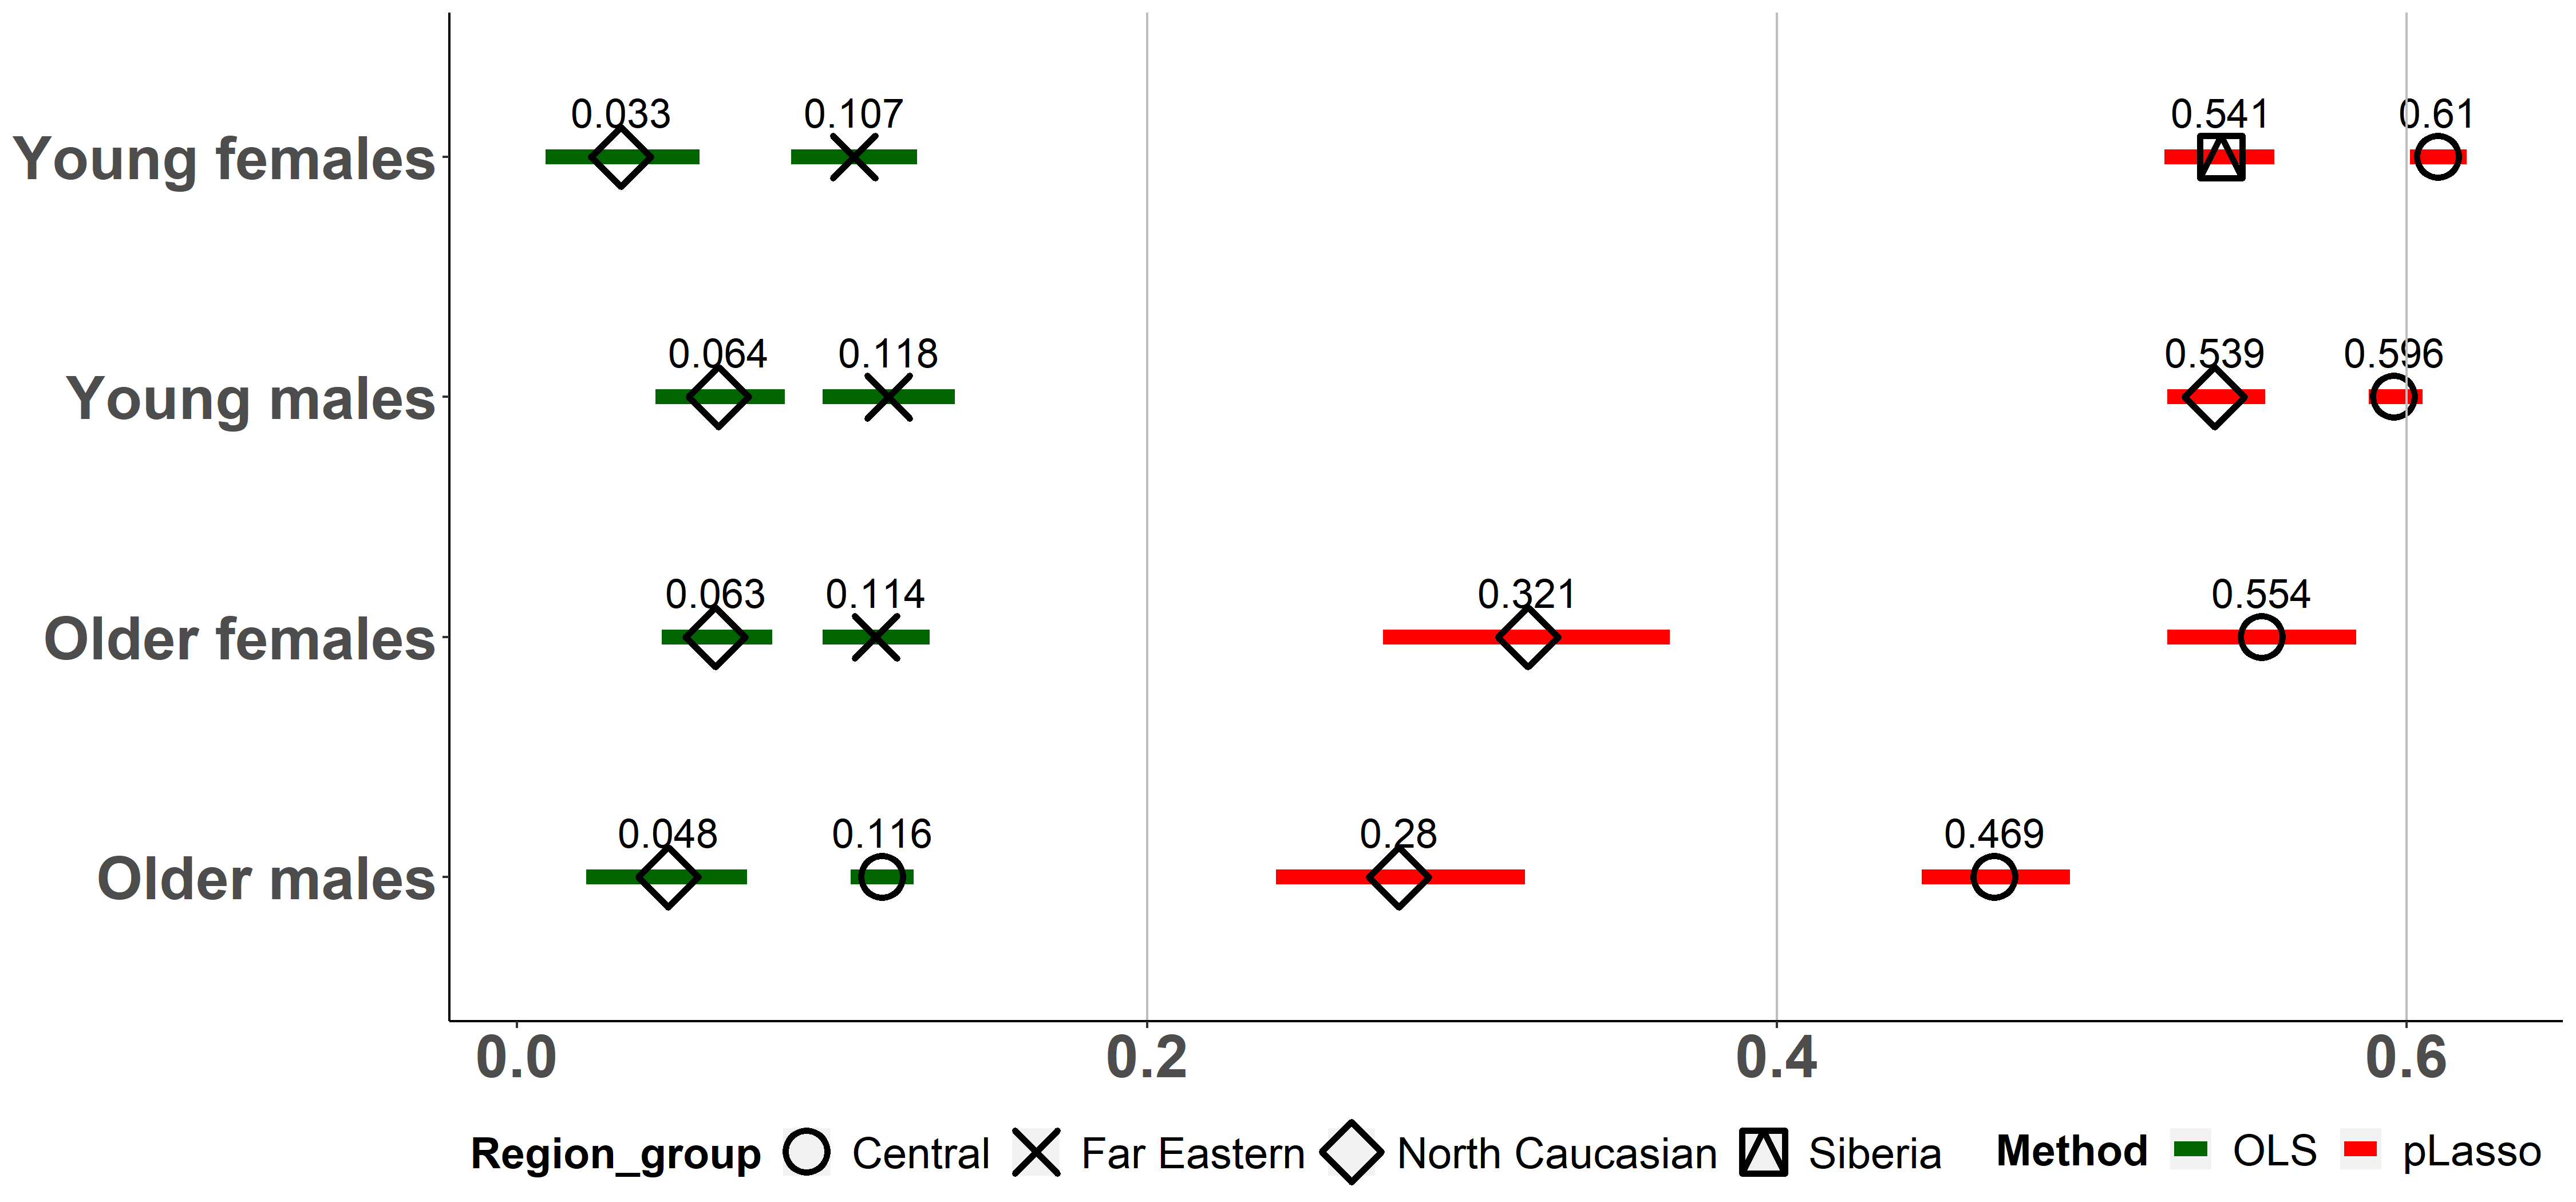
\includegraphics[width=\textwidth]{iv_by_districts.png}
	\caption{Returns to Education Estimates and 95\% CIs for Post-Lasso and OLS by Cohorts and\\
    Federal Districts (Maximum and Minimum for each Method), 2018} \label{fig:5.5}
\end{figure}

\newpage

\section{Conclusions}

\lipsum[1]



\printbibliography

\newpage
\section*{Appendix}




\newpage
\printbibliography

\end{document}
